\documentclass[a4paper]{llncs}

%\usepackage{amssymb}
%\setcounter{tocdepth}{3}
\usepackage{graphicx}

%\usepackage[linesnumbered,ruled,vlined]{algorithm2e}


\usepackage[colorlinks=true,
urlcolor=blue,
citecolor=blue,
linkcolor=blue,
           bookmarks=false,
           bookmarksnumbered,
           linktocpage=true
           ]{hyperref}

\usepackage{url}

% \urldef{\mailsa}\path|{alfred.hofmann, ursula.barth, ingrid.haas, frank.holzwarth,|
% \urldef{\mailsb}\path|anna.kramer, leonie.kunz, christine.reiss, nicole.sator,|
% \urldef{\mailsc}\path|erika.siebert-cole, peter.strasser, lncs}@springer.com|    
% \newcommand{\keywords}[1]{\par\addvspace\baselineskip
% \noindent\keywordname\enspace\ignorespaces#1}

%\usepackage{tikz}
%\usepackage{aeguill}
%\usepackage{tikzscale}
%\usepackage{filecontents} 
\usepackage{subfig}
\usepackage[font=small]{caption}

\usepackage{times}

\usepackage{color}

\newcommand{\mypara}[1]{\vspace{4pt}\noindent\textbf{#1}}
\newcommand{\mytt}[1]{\ensuremath{\mathtt{#1}}}


\begin{document}

\mainmatter  % start of an individual contribution

% first the title is needed
\title{DataONE: A Data Federation with Provenance Support}

% \author{Yang Cao\inst{1} \and Christopher Jones\inst{2} \and V\'ictor Cuevas-Vicentt\'in\inst{3} \and Steve Aulenbach\inst{4} \and Matthew B.\ Jones\inst{2} \and Bertram Lud\"ascher\inst{1} \and Timothy McPhillips\inst{1} \and Paolo Missier\inst{5} \and  Christopher Schwalm\inst{6} \and Peter Slaughter\inst{2} \and Dave Vieglais\inst{2} \and Lauren Walker\inst{2} \and Yaxing Wei\inst{7}}

\author{Yang Cao\inst{1},  Christopher Jones\inst{2},  V\'ictor Cuevas-Vicentt\'in\inst{3},  Steve Aulenbach\inst{4},  Matthew B.\ Jones\inst{2},  Bertram Lud\"ascher\inst{1},  Timothy McPhillips\inst{1},  Paolo Missier\inst{5},   Christopher Schwalm\inst{6},  Peter Slaughter\inst{2},  Dave Vieglais\inst{2},  Lauren Walker\inst{2}, Yaxing~Wei\inst{7}}


\institute{Library and Information Science, University of Illinois, Urbana-Champaign, IL\\
\and
National Center for Ecological Analysis and Synthesis, UCSB, CA \\
\and
Universidad Popular Aut\'onoma del Estado de Puebla, Mexico\\
\and
%University Corporation for Atmospheric Research and U.S.\ Global Change Research Program \\
UCAR and U.S.\ Global Change Research Program \\
\and
School of Computing Science, Newcastle  University, UK \\
\and
Woods Hole Research Center, Falmouth, MA \\
\and
Environmental Sciences Division, Oak Ridge National Laboratory, TN}



%
% NB: a more complex sample for affiliations and the mapping to the
% corresponding authors can be found in the file "llncs.dem"
% (search for the string "\mainmatter" where a contribution starts).
% "llncs.dem" accompanies the document class "llncs.cls".
%

\toctitle{Lecture Notes in Computer Science}
\tocauthor{Authors' Instructions}
\maketitle


\begin{abstract}
  DataONE is a federated data network focusing on earth and environmental science data.  We demonstrate new provenance capabilities that have been added to DataONE toolkit to facilitate reproducible research. A user, say ``Alice'', can annotate a (Matlab, R, Python, etc.) script using the YesWorkflow (YW) tool to describe the underlying workflow or \emph{prospective} provenance. After Alice has run the script, the result files, script, prospective provenance, and \emph{retrospective} provenance, represented in the ProvONE provenance model, can be bundled into an OAI-ORE compliant data package and uploaded to the DataONE network. A second user (``Bob'') can discover and access Alice's package and use her data for his own experiments. We show that Bob's results, once published through DataONE, link back to Alice's outputs via unique identifiers. Thus, a third user (``Charlie'') who browses DataONE will be able to discover the full provenance of Bob's results, all the way back to Alice's original contributions.  DataONE provenance systems enable reproducible research and facilitate proper attribution of scientific results transitively across generations of derived data products.  \end{abstract}

% \keywords{We would like to encourage you to list your keywords within
% the abstract section}



\section{Introduction}

DataONE (Data Observation Network for Earth) is a federated data network and a sustainable cyberinfrastructure for open, persistent, robust, and secure access to well-described and easily discovered Earth observational data~\cite{dataone}. The five primary goals of DataONE are: discovery and access, data integration and synthesis, education and training, building community, and data sharing. The DataONE infrastructure consists of three principal component:


\mypara{(1) Member Nodes} are existing or new data repositories that support the DataONE Member Node APIs.  A Member Node (MN) that implements anonymous, read-only access to data and metadata operates at the Tier-1 API level. This enables discovery of all objects available on the MN, low level description of each object, retrieval of the object given its identifier, and activity reporting. MNs also provide science metadata and relationships between metadata and data using resource maps \cite{oaiore} to facilitate discovery through DataONE Search.  Data repositories can also implement higher tiers of the DataONE API, including authentication and restricted data access (Tier-2), write access to storage resources (Tier-3), and replication of data from other nodes
% in the network
(Tier-4).


\mypara{(2) Coordinating Nodes} serve data management and discovery needs of the network. Services of a Coordinating Node (CN) include network-wide indexing of data objects, coordination of data replication between MNs, mirrored content of \emph{science metadata} (detailed descriptions of science data objects and collections) and \emph{system metadata} (low level metadata, e.g., data type, size, ownership, location) present at MNs.


\mypara{(3) Investigator Toolkit.} The Investigator Toolkit (ITK) contains user tools that enable interaction with DataONE infrastructure through a REST service API exposed by the CNs and MNs. Python and Java libraries are available for application developers, and DataONE support is present in scientific analysis tools such as Matlab and R.


The DataONE infrastructure was released for public use in 2012 and supports identifier resolution, content search and retrieval, the federated identity management infrastructure, and the replication service.

%\subsection*{DataONE Search}

\mypara{DataONE Search} is a web-based application allowing users to seamlessly and efficiently discover publicly accessible data packages within the DataONE federated network of Member Node repositories. It was released in November 2015, and allows users to search by map, dates, keywords and other facets and to refine the results using further parameters. Users can sign in to DataONE Search using ORCID credentials, Google accounts, and institutional accounts.

The software has been designed to facilitate rapid iteration and deployment of new features and to take full advantage of future capabilities offered by upcoming versions of the core cyberinfrastructure. Notable among these is the \emph{provenance information} within search and discovery. In the next section, we will demonstrate new DataONE provenance tools and the visualization of provenance with DataONE Search.


\section{Demonstration Description}  \label{demo}

DataONE has developed a \emph{Run Manager} for capturing provenance from R \cite{recordr} and Matlab \cite{matlabdataone} script executions, and contributed to the development of YesWorkflow \cite{yesworkflow} to provide an improved understanding of a script in terms of its user-declared workflow structure and system-recorded file I/O. The automatic capture of the latter is transparent to scientists and provides medium-grained\footnote{unlike the fine-grained provenance captured, e.g., by noWorkflow \cite{nw14}} provenance by focusing on file I/O events.

We will use an example to introduce the core provenance and search features of DataONE. Suppose that Alice is an earth scientist whose work involves generating global grass fraction maps from water, air temperature, and other input data. Bob is a scientist who runs a grassland water use efficiency analysis built upon Alice's output. Charlie is a user of DataONE.

\subsection{User Alice's view: Local Run Manager View}

%\begin{figure}
%\centering   
%\subfloat[YesWorkflow annotations example used in Alice's script which annotate a block of code with input and output information \label{yw}]{%
%      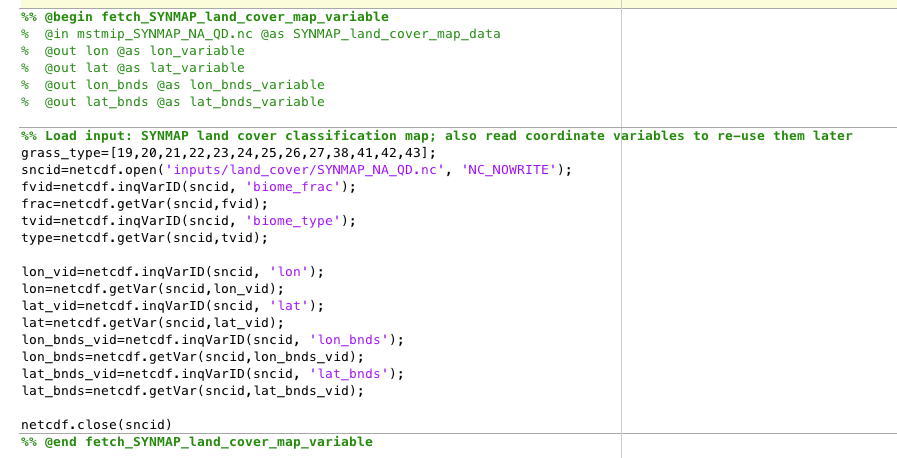
\includegraphics[width=0.5\textwidth, height=2in]{yw-annotations}
%  }
%\subfloat[Alice calls the record() function to record a run for her script \label{record-snapshot}]{%
%      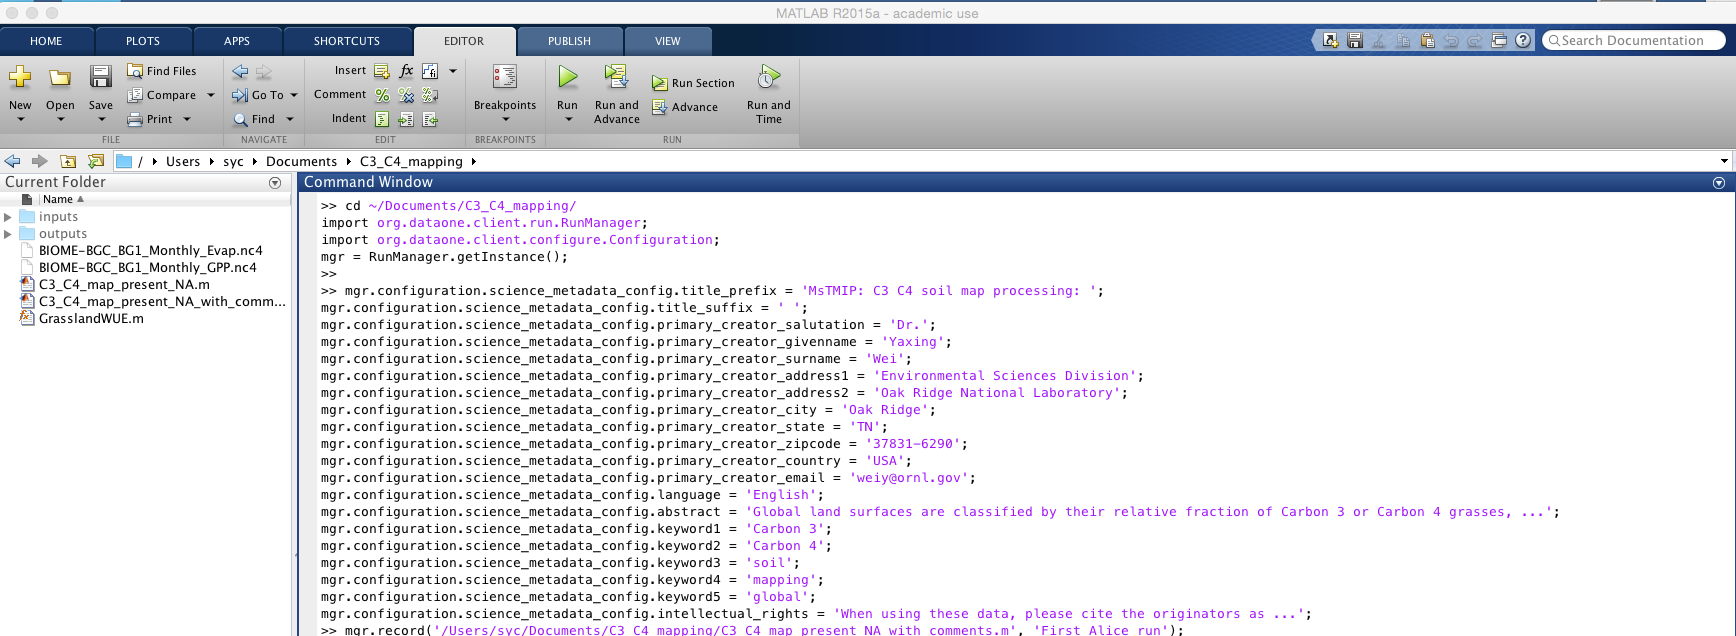
\includegraphics[width=0.5\textwidth, height=2in]{record_Alice_run}
% }
% \\
% \subfloat[Alice calls the view() function to check the recorded execution information \label{view-snapshot}]{%
%      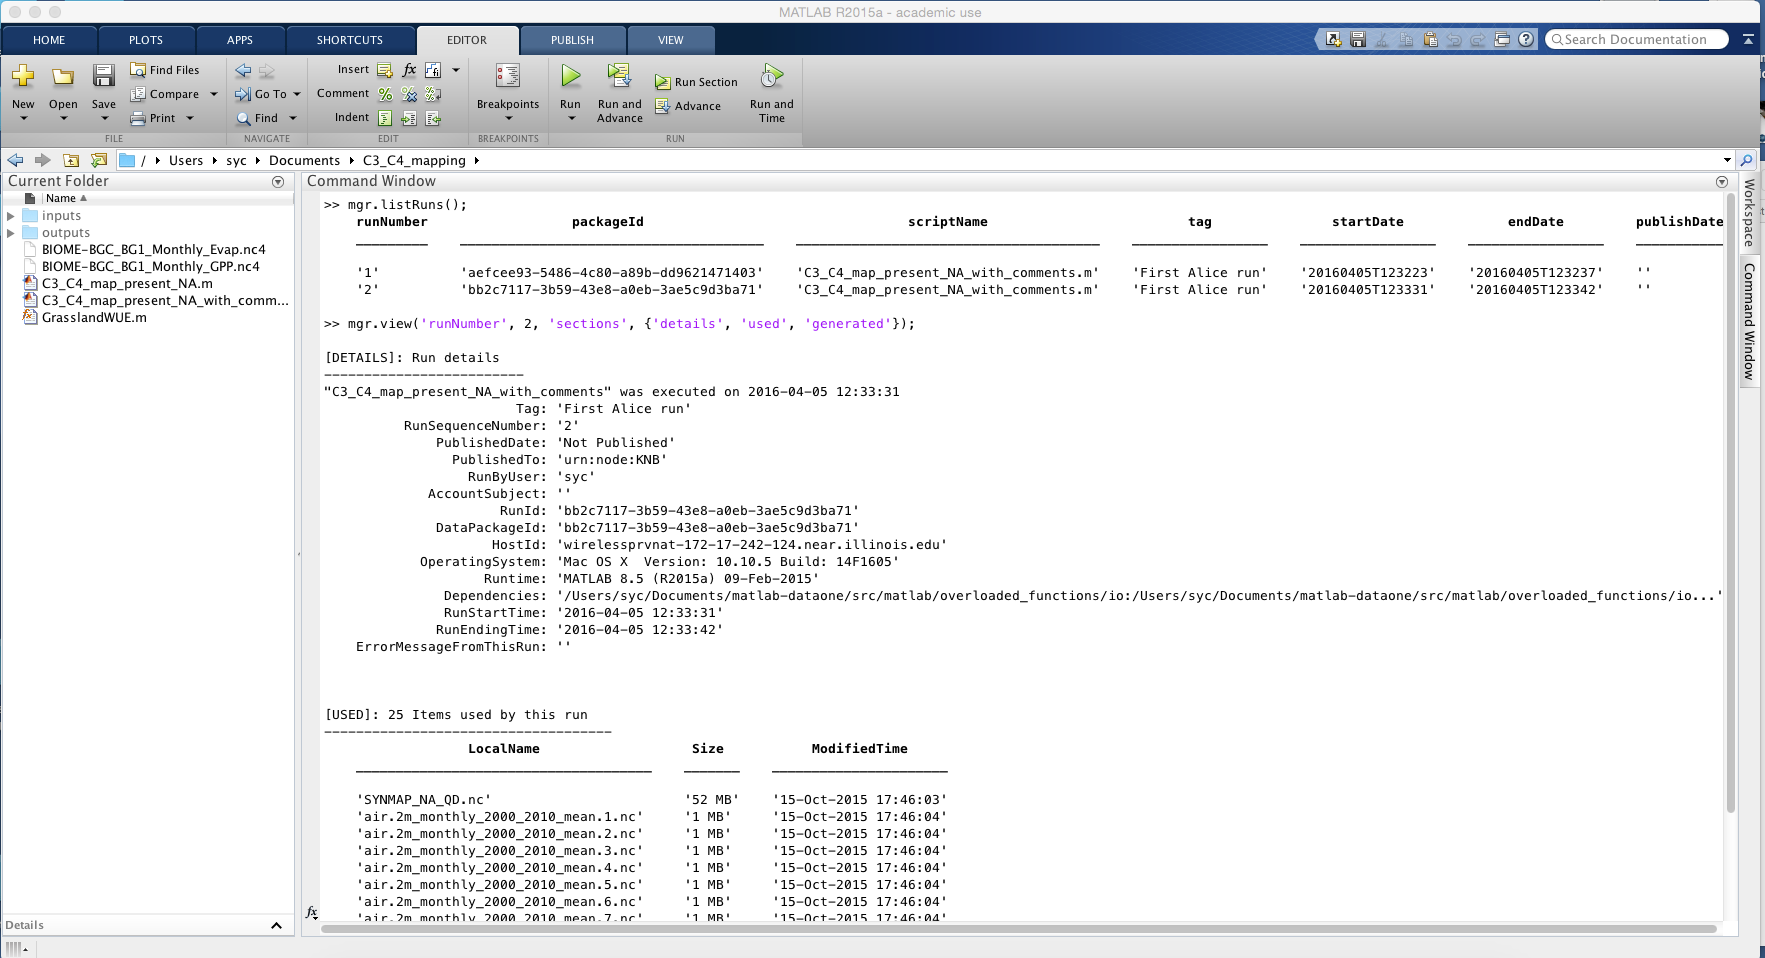
\includegraphics[width=0.5\textwidth, height=2in]{view_Alice_run}
% }
% \subfloat[Alice calls the publish() function to share her execution and data with others to DataONE network \label{publish-snapshot}]{%
%      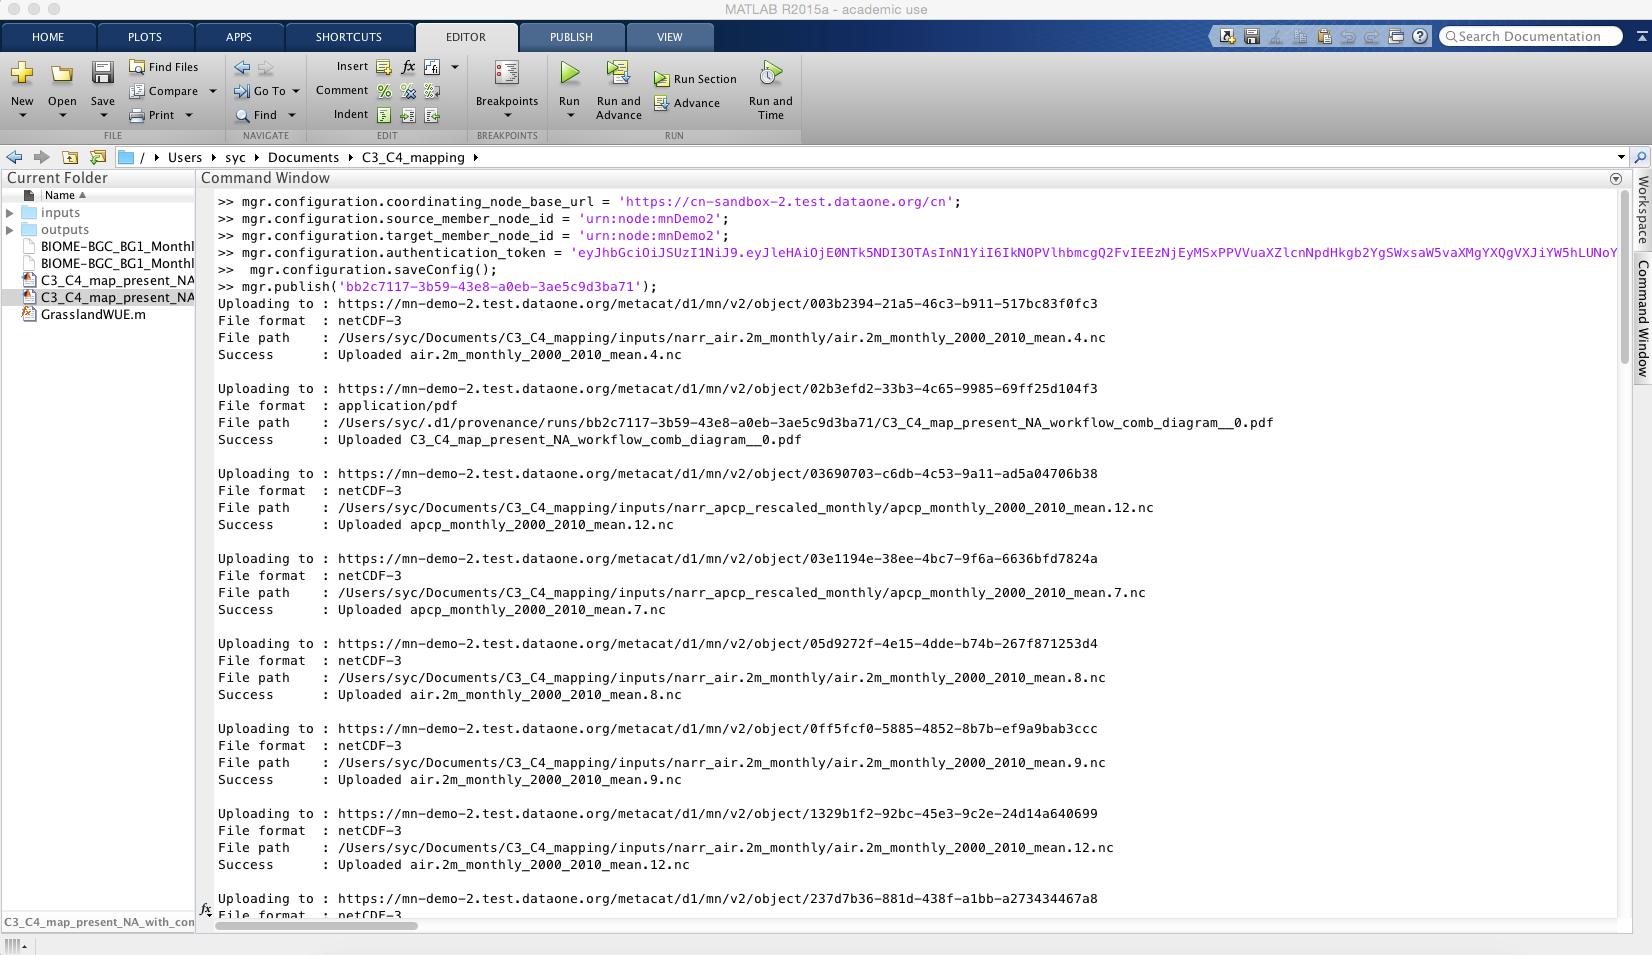
\includegraphics[width=0.5\textwidth, height=2in]{publish_Alice_run}
% }
% \caption{Snapshots when Alice uses DataONE Provenance tool to annotate her script steps, record the execution of her script, view the details for one run, and publish her run to the DataONE network.}
%\label{fig0}
%\end{figure}

%\begin{figure}[t] \centering 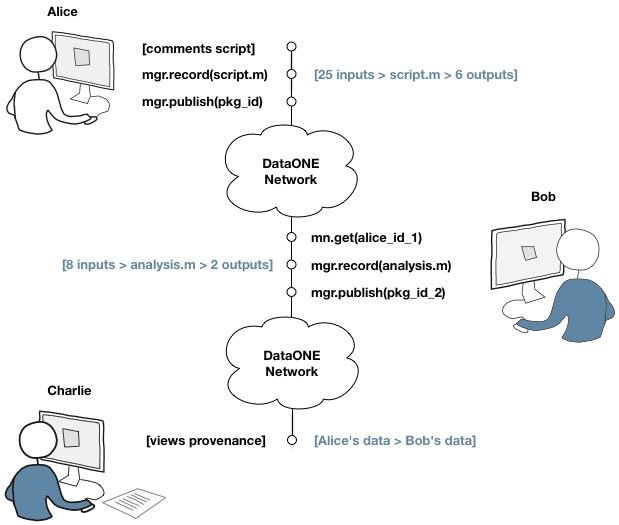
\includegraphics[width=0.5\textwidth]{alice-bob-charlie-sequence} \caption{Run Manager Demonstration: (1) Alice runs \mytt{script.m} with the DataONE Run Manager to create data package $P_A$, which she publishes to the DataONE network; (2) Bob later finds and downloads Alice's data, uses it in his \mytt{analysis.m}, creating and then publishing package $P_B$; (3) Charlie searches DataONE, finds Bob's $P_B$, and recognizes its dependence on Alice's $P_A$.}  \label{fig0} \end{figure}

\begin{figure}[t] \centering 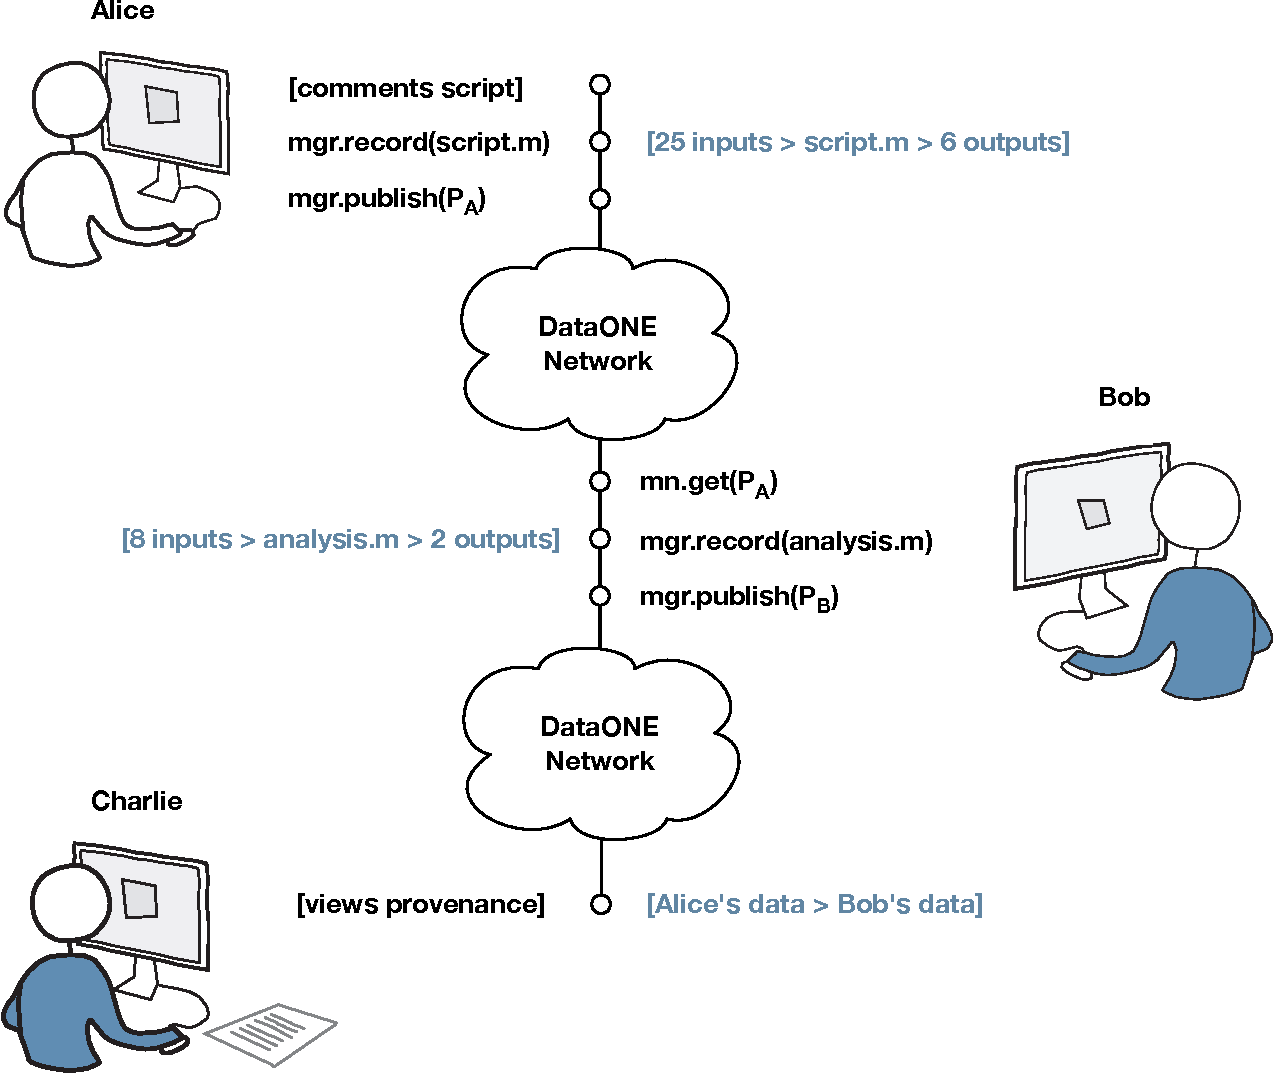
\includegraphics[width=0.4\textwidth]{figs/alice-bob-charlie-sequence-crop} \caption{Run Manager Demonstration: (1) Alice runs \mytt{script.m} with the DataONE Run Manager to create data package $P_A$, which she publishes to the DataONE network; (2) Bob later finds and downloads Alice's data, uses it in his \mytt{analysis.m}, creating and then publishing package $P_B$; (3) Charlie searches DataONE, finds Bob's $P_B$, and recognizes its dependence on Alice's $P_A$.}  \label{fig0} \end{figure}

In Figure~\ref{fig0}, Alice has developed a script for producing Carbon3/Carbon4 soil maps.  She uses the YesWorkflow (YW) tool to mark-up the script and expose the underlying workflow view (i.e., prospective provenance) that is inherent in her carbon mapping code. Alice then runs her script using \emph{Run Manager} (the DataONE provenance capture tool) in Matlab. After a couple of runs, Alice is happy with the results and publishes them to the DataONE network. To do so, she bundles up the data results along with the runtime (retrospective) provenance captured by the DataONE Matlab provenance recorder, the script itself and its YW-generated workflow view.

\textcolor{red}{The DataONE Matlab tool facilitates her work by generating the DataONE-compliant data package in OAI-ORE format, including the provenance information in ProvONE format as part of the package. ProvONE~\cite{provone} is an extension of the W3C PROV-O~\cite{prov-o} standard for representing provenance, and includes specializations for representing both retrospective provenance about the runtime execution and prospective provenance about the structure and flow of the analytical script or workflow.}


When using DataONE Search with the keyword ``grass'', Bob finds Alice's data package \cite{yaxing}. Bob uses outputs from Alice for his own study, which he also shares via DataONE. Since he used the unique identifiers from Alice's outputs, the provenance traces produced by Alice's and Bob's runs are naturally \textcolor{red}{connected through} the nodes that carry those data identifiers. Charlie discovers Bob's data packages on DataONE and is able to navigate back to the data that Bob used, i.e., Alice's data package depicted in Figure~\ref{fig2}~\cite{Katz,data-trajectories}.


\subsection{User Bob's view: Local Run Manager View}

When Bob searches for data in DataONE and finds Alice's data and code, he uses the Matlab Toolbox to fetch the data in a way that is identifier-aware, rather than having to manually maintain the provenance information. For example, he calls the \mytt{MemberNode.get}(session, identifier) function in his analysis script because this function has provenance tracking capabilities. Then, the Toolbox downloads the data and uses the same identifier to store the data locally. Additionally, a \emph{prov:used} statement that Bob is using Alice's data is recorded.

When Bob then calls \mytt{publish}() to upload his scripts and data, data in his package that are not present in the DataONE network will be uploaded.  When all data are within the DataONE network, their respective provenance statements are indexed on the \emph{Coordinating Node}, and are available to be used in the web provenance display.



\subsection{User Charlie's View: DataONE Search Website}

When Charlie searches the keyword ``grass'' in the DataONE Search, two data packages are found and shown in Figure~\ref{fig1}. One data package is created by ``Alice'' (Yaxing Wei in the real world) \cite{yaxing}, the other is created by ``Bob'' (Christopher Schwalm) \cite{christopher}. Both data packages show that provenance information is associated with each dataset (via the icon in the search record) and can be seen at \textcolor{red}{within the} DataONE Search demo site \cite{dataone-demo}.

\begin{figure}[t]
\centering   
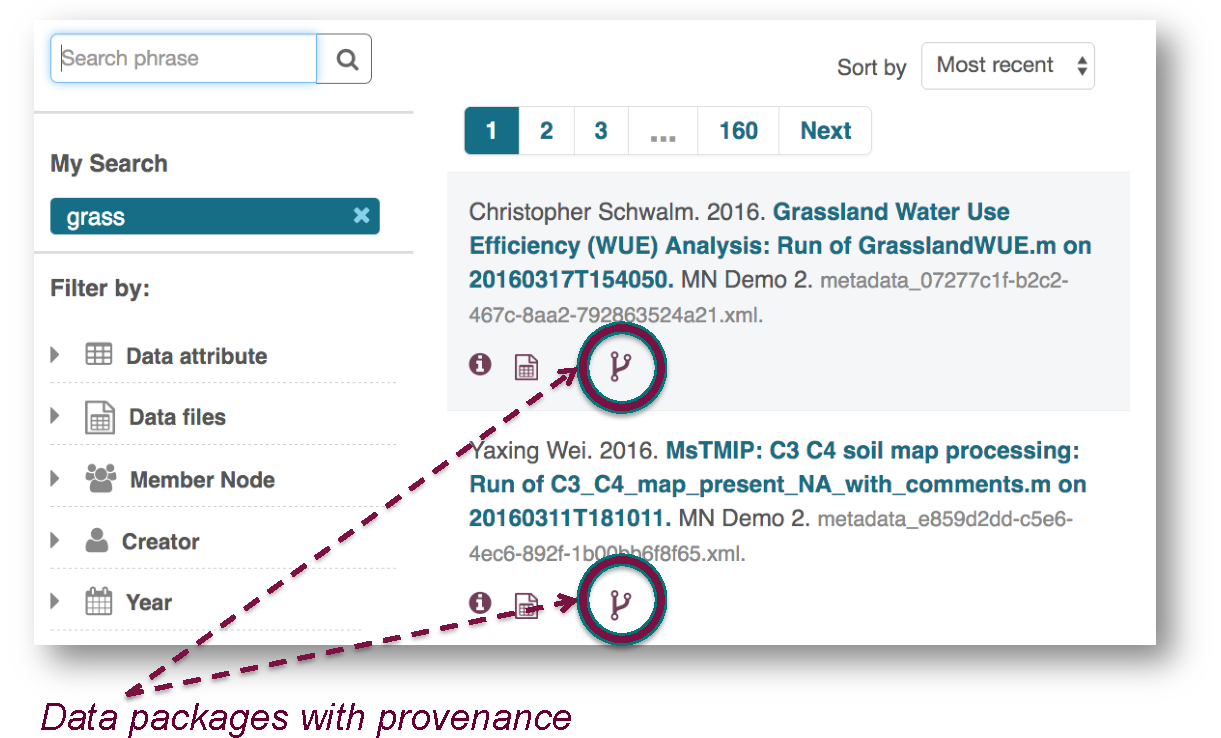
\includegraphics[width=0.6\textwidth]{figs/ab-crop}
\caption{DataONE Search result for keyword  ``grass'' (DataONE Search demonstration site). The ``fork'' icon indicates data packages having embedded provenance.}
\label{fig1}
\end{figure}

Prospective and retrospective provenance information can be explored from the DataONE Search site. Provenance details for any input or output in the provenance graph can be viewed by clicking on the icon shown on Figure~\ref{fig2}. DataONE Search provides human language descriptions of how data are used or generated via the script and models, and provides navigation \textcolor{red}{to ancestors and descendants in the data derivation chain}. Figure~\ref{fig2} shows two data packages produced by the execution of Alice and Bob's workflow scripts, and the provenance lineage between these two data packages. 

Alice's data package \cite{yaxing} is shown on the top layer of Figure~\ref{fig2}, created when Alice ran her script using the DataONE provenance capture tool, or Run Manager, in Matlab. Her script (C3\_C4\_map\_present\_with\_comments.m) takes twenty-five input files and produces six outputs, which are shown on the left side and right side of Alice's data package in Figure~\ref{fig2}, respectively. The bottom three outputs in Alice's data package are the NetCDF data files that represent three different world map grids of percentage of grass types (C3 grass fraction, C4 grass fraction, and total grass fraction). In addition, a model graph is displayed at the intermediate layer \textcolor{red}{that was generated by YesWorkflow tool}\cite{yesworkflow}. Alice's workflow script used embedded YesWorkflow annotations to document her script. These annotations declare step by step how data are used and derived in the script. 


Bob's data package \cite{christopher} created by DataONE provenance tool (Run Manager) is displayed at the bottom layer. When Bob browses Alice's data package on the DataONE Search site, he decides to use three NetCDF output data produced by Alice's work in his Grassland Water Use Efficiency Analysis script (GrasslandWUE.m). From the provenance information associated with Bob's data package in Figure~\ref{fig2}, we see that it takes eight inputs, and produces two visualizations. By viewing the details for each input, we can see that three of them are the outputs produced by Alice's data package.  

In order to maintain the link between the outputs from Alice's data package to the inputs to Bob's package, Bob needs to use the same identifier in his script as Alice does. An alternative approach is that Bob creates a new identifier when he downloads Alice's data. However, the link between two data packages will be broken which has been discussed in \cite{missing-link}.  

\begin{figure}[t]
\centering   
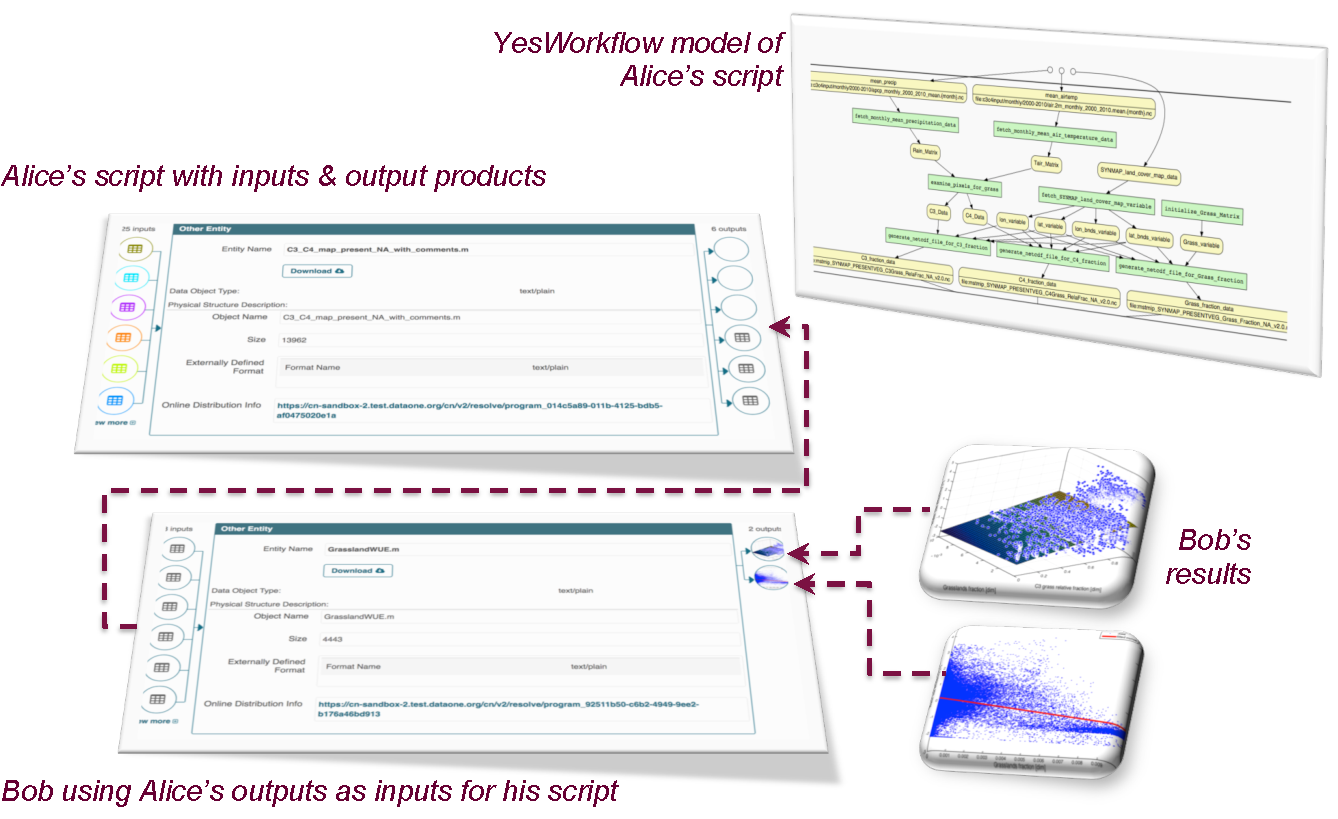
\includegraphics[width=0.8\textwidth]{figs/abc-crop}
\caption{Charlie's view on the DataONE demo site: (1) A YesWorkflow model for Alice's soil processing script; (2) Data lineage from Bob's results back through his script inputs to Alice's data package; (3) Two visualizations produced by Bob's water use efficiency analysis script.}
\label{fig2}
\end{figure}


\section{Discussion and future work}

This paper demonstrates a notable new feature (provenance capture and search) of DataONE. DataONE has released the DataONE Search for public use in November 2015, and the R and Matlab provenance tool to the public in 2016. 

Maintaining the link between Alice's work and Bob's subsequent work is worth \textcolor{red}{discussion}. Currently, Bob must use certain functions provided by DataONE to \textcolor{red}{ensure} the provenance link to Alice's work \textcolor{red}{is} correctly maintained. There are other possible ways to achieve the same goal. For example,  Bob \textcolor{red}{might} download Alice's data and manually add the links to Alice's work back into his data package before sharing via DataONE. A \emph{prov:was\_derived\_from} statement that local data copy for Bob is derived from Alice's data \textcolor{red}{could} easily \textcolor{red}{add, especially for historical data for which provenance was not captured at the time data were generated.  The new provenance tools described in this demonstration allow efficient capture of machine-parseable provenance information using analytical tools commonly used in the environmental sciences (e.g., Matlab), thereby significantly improving the replicability of research in the environmental sciences.}


Future work of the current provenance tools include: (1) solve the broken link use case; (2) support more I/O functions; (3) handle complex scenarios such as multiple runs of a script and multiple users; (4) variable-level provenance capture warrants further investigation and efforts.



\begin{thebibliography}{4}
\small

\bibitem{christopher} Christopher Schwalm's DataPackage, \url{https://search-sandbox-2.test.dataone.org/#view/metadata_07277c1f-b2c2-467c-8aa2-792863524a21.xml}

\bibitem{yaxing} YaXing Wei's DataPackage, \url{https://search-sandbox-2.test.dataone.org/#view/metadata_e859d2dd-c5e6-4ec6-892f-1b00bb6f8f65.xml}

\bibitem{dataone} Data Observation Network for Earth (DataONE), \url{https://www.dataone.org}

\bibitem{dataone-demo} DataONE Search Demo Site, \url{https://search-sandbox-2.test.dataone.org}

\bibitem{matlabdataone} Jones C., Cao Y., Slaughter P., Jones M.: Matlab DataONE Toolbox. \url{https://github.com/DataONEorg/matlab-dataone} (2016)

\bibitem{Katz} Katz, D.S. \& Smith, A.M.: Implementing Transitive Credit with JSON-LD. Journal of Open Research Software. 3(1), p.e7. (2015) 

\bibitem{nw14} Murta, L., Braganholo, V., Chirigati, F., Koop, D., Freire, J.: noWorkflow:
  Capturing and analyzing provenance of scripts. In: International Provenance
  and Annotation Workshop (IPAW). pp. 71--83. Cologne, Germany (2014)

\bibitem{yesworkflow} McPhillips T., Song T., Kolisnik T., Aulenbach S., Belhajjame K., Bocinsky R.K., Cao Y., Cheney J., Chirigati F., Dey S., Freire J., Jones C., Hanken J., Kintigh K.W., Kohler T.A., Koop D., Macklin J. A., Missier P., Schildhauer M., Schwalm C., Wei Y., Bieda M., and Lud\"ascher B.: YesWorkflow: A User-Oriented, Language-Independent Tool for Recovering Workflow Information from Scripts. Intl.\  Journal for Digital Curation, 10, 298--313. (2015)

\bibitem{missing-link} Missier, P., Lud\"ascher, B., Bowers, S., Anand, M. K., Altintas, I., Dey, S., Sarkar, A., Shrestha, B. and Goble, C.: Linking Multiple Workflow Provenance Traces for Interoperable Collaborative Science.  In: 5th Workshop on Workflows in Support of Large-Scale Science. (2010). 

\bibitem{data-trajectories} Missier, P.: Data Trajectories: Tracking Reuse of Published Data for Transitive Credit Attribution. In: 11th International Data Curation Conference. (2016). 

\bibitem{recordr} Slaughter P., Jones M., Jones C.: NCEAS recordr: Provenance tracking for R. \url{https://github.com/NCEAS/recordr} (2016)

\bibitem{oaiore} Open Archives Initiative Object Reuse and Exchange, \url{https://www.openarchives.org/ore/}

\bibitem{provone} ProvONE: A PROV Extension Data Model for Scientific Workflow Provenance, \url{https://purl.dataone.org/provone-v1-dev}

\bibitem{prov-o} W3C PROV-O: The PROV Ontology, \url{https://www.w3.org/TR/prov-o/}



\end{thebibliography}


\end{document}
